\chapter{MBE multiplier}
A speedup of the second stage of the floating point multiplier can be achieved by adopting a modified Booth enconding architecture. It resorts to the booth encoding implemented in a fully parallel structure where all partial products are generated by means of combinational blocks. 
\section{Structure and algorithm}
The multiplier is made up of three parts:
\begin{itemize}
	\item Partial products computation
	\item Multioperand adder based on a Dadda tree
	\item Two-operand adder
\end{itemize}
A strategy aimed at minimizing the tree height is put in place as suggested.
This optimization makes the hardware description non-trivial, since standard \texttt{generate} statements do not readily provide a solution to parametrize this irregular structure given the bitwidth. 
The preferred approach has been that of using a Matlab script to compute the number and location of all full-adders and half-adders adopting the rules specific to Dadda trees. The outcome is then translated into VHDL code by directly declaring all the needed signals and instantiating components (whose number may grow large in the case $N=32$ or $N=24$).
The first step in designing a Dadda tree is to find the least integer $J$ such that $d_J > N$, where 
\begin{equation*}
d_j = \left \lfloor{\frac{3}{2}d_{j-1}}\right \rfloor \hspace{1cm}\,\,d_1 = 2
\end{equation*}
The core of the algorithm is best understood with the aid of the \textit{dot representation}. The tree will include several stages (indexed by $j=J, J-1, ..., 2$) where bits of each operand are represented by dots and are suitably aligned in a matrix. For each stage $j$ (starting from $J$) the algorithm runs along the columns allocating the least resources with the aim of having no more than $d_{j-1}$ dots in the next stage labeled $j-1$. In the following $n_j^i$ is the number of dots allocated in column $i$ within stage $j$, $a_j^i$ is the number of full-adders in column $i$, $b_j^i$ is the number of half adders, $c_j^i$ is the number of remaining dots, which are copied to the next stage.

\begin{algorithmic}
	\FOR{$j = J-1$ \textbf{downto} $1$} 
		\FOR{$i=1$ \TO $2N$}
		\STATE {$k=d_j-n_j^i$}
		\IF{$n_{j+1}^i < k$}
			 \STATE {$a_{j+1}^i=0$}
			 \STATE {$b_{j+1}^i=0$}
		\ELSIF{$(n_{j+1}^i - k)\,\textrm{mod}\, 2 = 0$ }
			\STATE {$a_{j+1}^i=(n_{j+1}^i - k)/2$}
			\STATE {$b_{j+1}^i=0$}
		\ELSE
			\STATE {$a_{j+1}^i=\left\lfloor{ (n_{j+1}^i - k)/2} \right \rfloor$}
			\STATE {$b_{j+1}^i=1$}
		\ENDIF
		\STATE {$c_{j+1}^i=n_{j+1}^i-3a_{j+1}^i-2b_{j+1}^i$} \textit{ Remaining dots}
		\STATE $n_j^i = n_j^i + a_{j+1}^i + b_{j+1}^i + c_{j+1}^i$ \textit{Place sum bits in the corresponding column of the next stage}
		\STATE $n_j^{i+1} = a_{j+1}^i + b_{j+1}^i$ \textit{Place carry bits in the next column to the left}
		\ENDFOR
	\ENDFOR
\end{algorithmic}

Once the matrices $a$ and $b$ are available, writing VHDL code automatically to instantiate the required number of full adders is a simple matter.


\subsection{Testbench} Given the complexity of this block, individual testing is recommended so as to ensure that this component can be safely inserted as a sub-unit in a larger design. A fully automated testbench based on random numbers is available in \texttt{src/MBE/}.

\section{Synthesis}

\begin{figure}
	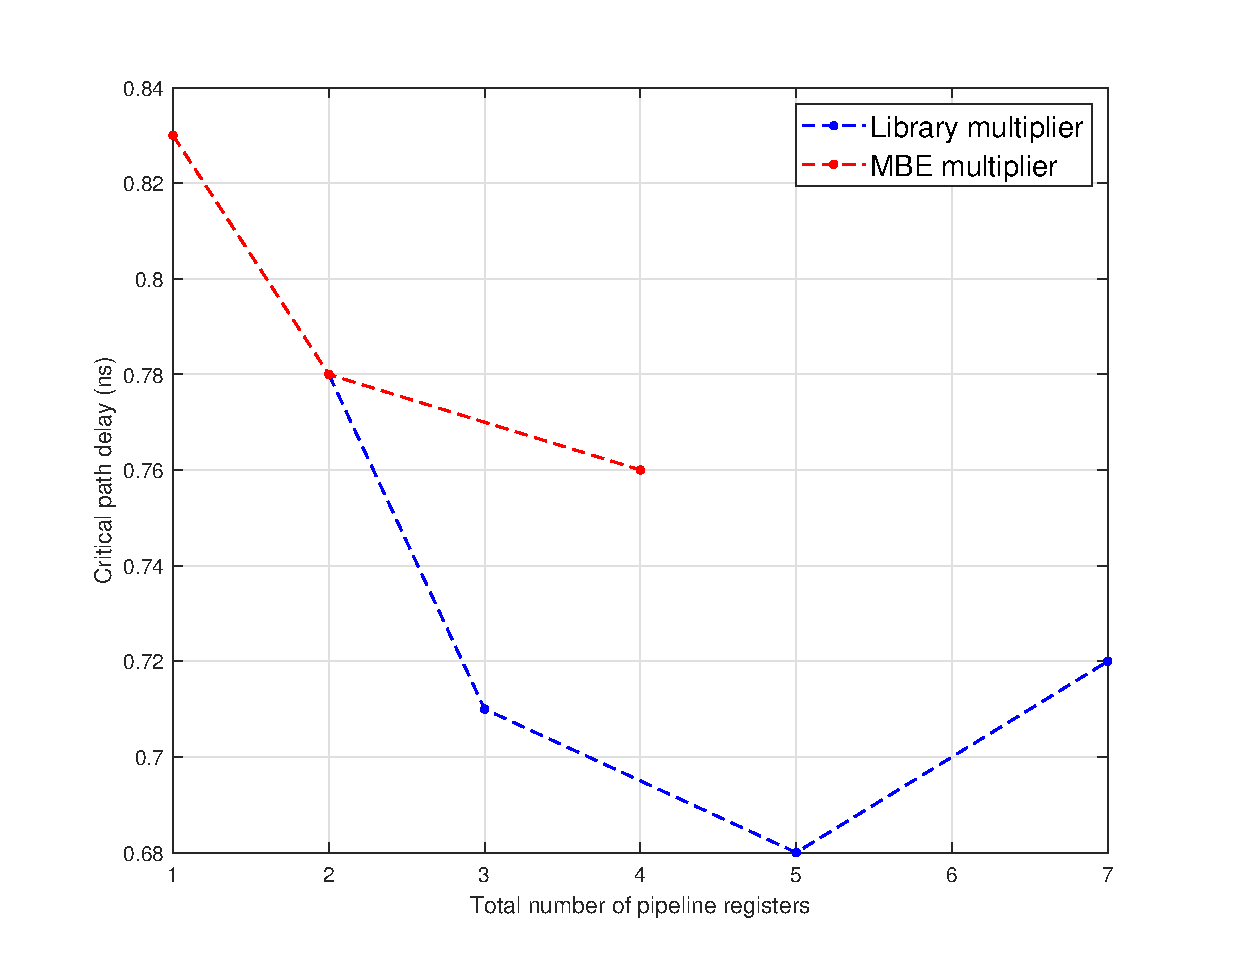
\includegraphics[width=\textwidth]{chapter2/images/delays.eps}
	\caption{Critical path delays as a function of total number of pipeline registers}
	\label{fig:delays}
\end{figure}
This new multiplier replaces the library multiplier instantiated in the second stage of \texttt{fpmul}. In order to fairly assess the impact that this component has on performance, pipeline registers are included and the synthesis process is repeated with several values of \texttt{NPIPE}, the constant denoting the number of pipeline registers.
\begin{table}
\begin{tabular}{|l|l|l|l|l|l|l|}\hline
	& No retiming & \texttt{NPIPE=1} & \texttt{NPIPE=2} & \texttt{NPIPE=4} & \texttt{NPIPE=6} & \texttt{NPIPE=8}\\\hline
	Clock period & 1.44$\,\textrm{ns}$ & 0.83$\,\textrm{ns}$& 0.78$\,\textrm{ns}$& 0.76$\,\textrm{ns}$ & 0.71 $\,\textrm{ns}$& 0.68$\,\textrm{ns}$ \\\hline
	Area (total) & 5935 & 6926 & 7130 & 7992 & 8402 & 8273 \\\hline
	Area (combinational) & 4794 & 4842 & 4655 & 4749 & 4729 & 4657 \\\hline
	Area (\texttt{mbe\_mult/add\_1424}) & 372 (6.3 \%)  & 419 (6 \%)  &  705 (9.9 \%)& 654 (8.2 \%) & 648 (7.7 \%) & 643 (7.8 \%)\\\hline
\end{tabular}
\caption{Characterization of the MBE multiplier}
\label{tab:MBE}
\end{table}
\autoref{fig:delays} shows that the MBE multiplier can potentially reach the same critical path delay as the library one, provided that more pipeline stages are inserted. This plot shows that there is an optimum number of pipeline stages, beyond which it is no longer possible to break critical paths using this technique. The MBE design reaches the minimum critical path delay with eight registers, whereas four stages are the best choice when resorting to the DesignWare component. Designs that include the MBE multiplier have been synthesized using a larger total area, as apparent by comparing \autoref{tab:MBE} with \autoref{tab:stage2}.
